\documentclass{beamer}

\usepackage[utf8]{inputenc}
\usepackage{default}
\usepackage{graphicx}
\usepackage{epstopdf}
\graphicspath{ {imagenes/} }

\usetheme{Warsaw}
\usecolortheme{crane}
\useoutertheme{shadow}
\useinnertheme{rectangles}

\title{Binomial Heap}

\author{Chris Chávez}
\institute{Universidad Nacional de San Agustín - Escuela Profesional de Ciencias de la Computación}
\date{\today}

\begin{document}

\frame{\titlepage}

\begin{frame}
 \frametitle{Binomial Heap}
 \begin{itemize}
  \item El Binomial Heap es una extensión del Binary Heap
	que proporciona una operación unión más rápida y ejciciente,
	además de fusionar esta operación con otras acciones previstas
	por el Binary Heap.
  \item El Binomial Heap es una colección de árboles Binomiales.
 \end{itemize}
\end{frame}

\begin{frame}
 \frametitle{Binomial Tree}
 \begin{itemize}
  \item Un árbol Binomial de orden 0 tiene 1 nodo.
  \item Un árbol Binomial de orden k se puede construir recusivamente mediante la unión de dos
	      árboles binomiales de orden k-1. Poniendo uno como hijo más a la izquierda del otro. 
 \end{itemize} 
\end{frame}
\begin{frame}
 \frametitle{Características}
 \begin{itemize}
    \item Tiene exactamente $2^{k}$ nodos.
    \item Tiene una altura k.
    \item Hay exactamente $\binom {k} {i}$ nodos en la altura i,
	  donde i = 0,1,...,k.
    \item La raiz tiene grado k y los hijos son árboles binomiales con
	  orden k-1, k-2,...0 de izquierda a derecha.
 \end{itemize}
\end{frame}

\begin{frame}
 \begin{figure}
  \centering
  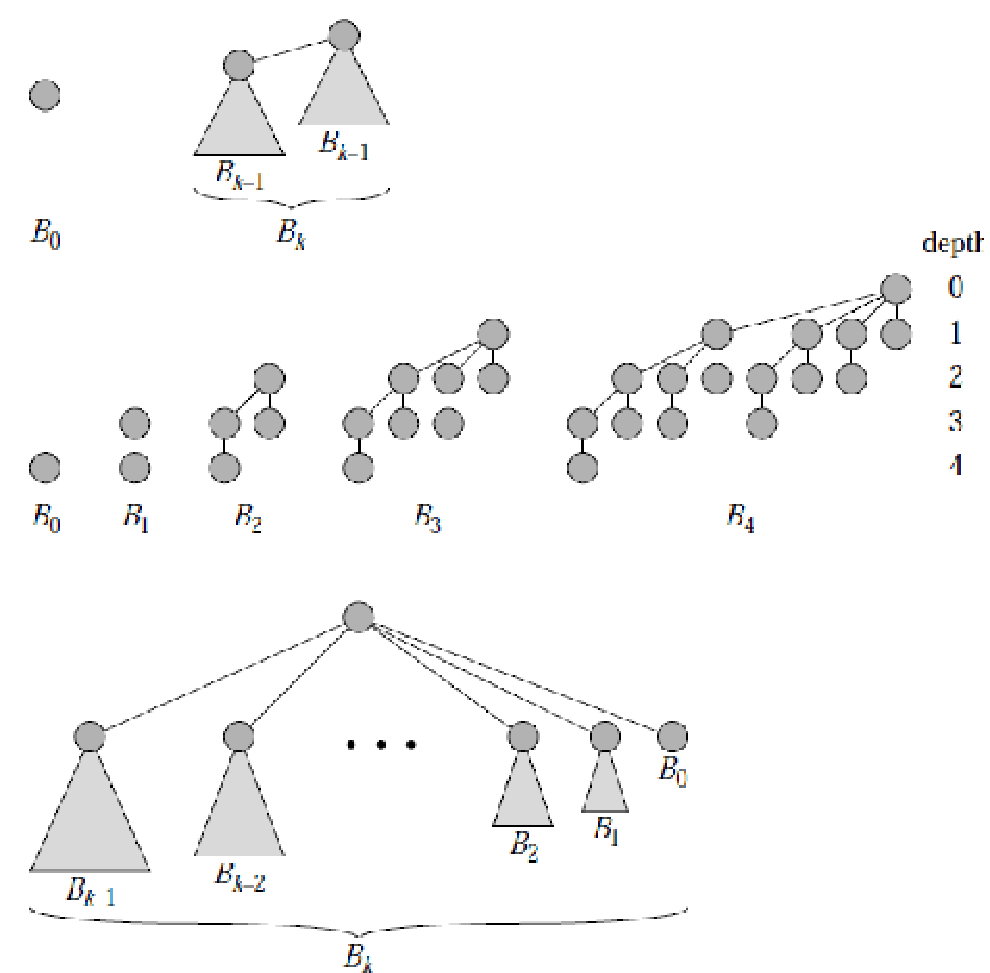
\includegraphics[scale = 0.5]{1.pdf}
  \label{img1}
 \end{figure}
\end{frame}

\begin{frame}
 \frametitle{Binomial Heap}
 \begin{itemize}
  \item Un Binomial Heap es un conjunto de árboles Binomiales,
	donde cada árbol Binomial sigue las propiedades de un Min Heap (o max Heap).
  \item Sólo puede haber a lo sumo un arbol binomial de cualquier orden.
 \end{itemize}
 \begin{figure}
  \centering
  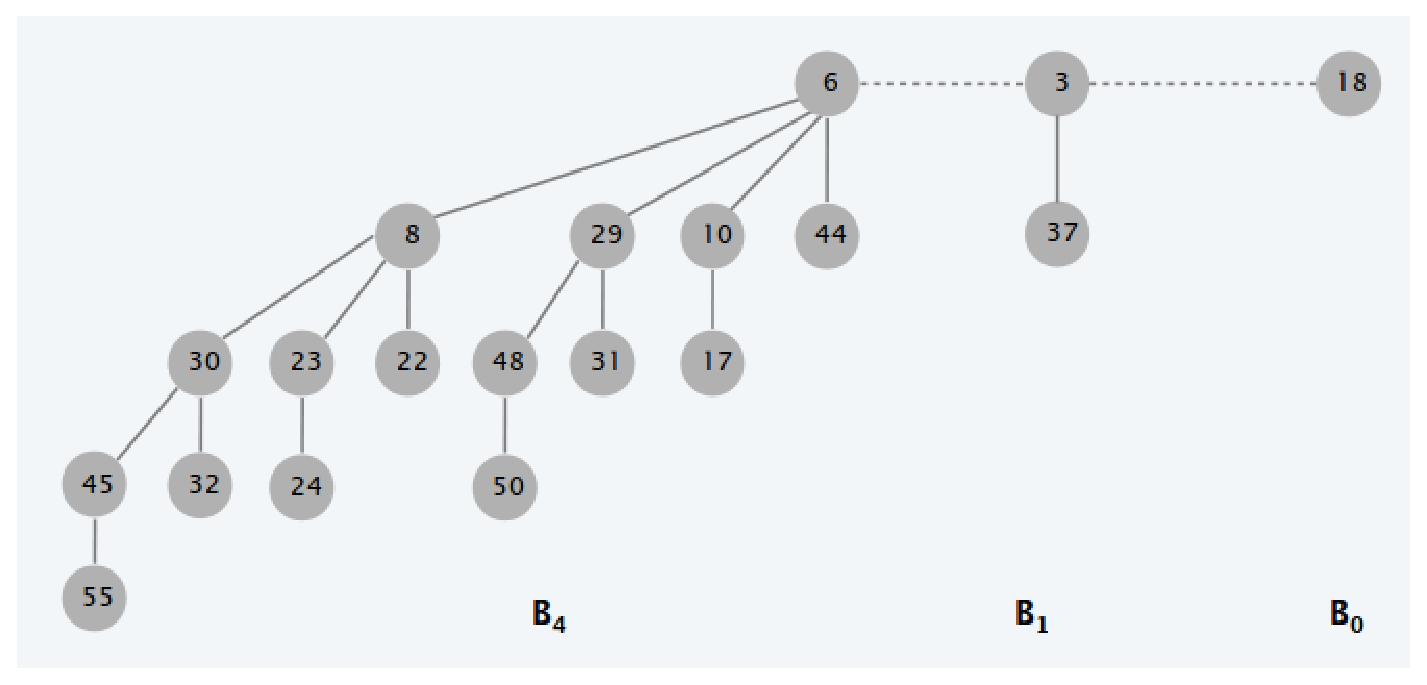
\includegraphics[scale= 0.4]{2.eps}
 \end{figure}
\end{frame}

\begin{frame}
 \frametitle{Representación binaria de un número con Binomial Heaps}
 Un Binomial Heap con \textbf{n} nodos tiene el número de árboles binomiales
 igual al número de bits \textbf{1} en la representación binaria del número \textbf{n}.
 También podemos relacionar el orden de estos árboles binomiales con las posiciones de
 dichos bits.
 Con esta relacion se puede concluir que: $$B \leq [\ln n] + 1$$
 Donde \textbf{B} es el número de árboles binomiales y \textbf{n} es el número de nodos del binomial Heap. 
\end{frame}

\begin{frame}
 \frametitle{Enlaces}
 \begin{itemize}
 \item El método típico de la implementación de los enlaces entre nodos es tener punteros a
 un padre, hermano e hijo. Un nodo no tiene enlace directo con todos sus hijos,
 sino que va a su primer hijo y luego itera a través de cada hermano.
 \item Las raices de los árboles binomiales se conenctan mediante un puntero a siguiente;
 como una lista simplemente enlazada.
 \end{itemize}
  \begin{figure}
   \centering
   \includegraphics[scale = 0.4]{3.eps}
  \end{figure}
\end{frame}

\begin{frame}
 \frametitle{Union}
 \begin{itemize}
  \item El primer paso es hacer un merge simple entre los dos Heaps
	en forma creciente.
  \item Después del merge, nosotros necesitamos asegurarnos de que no exista
	más de un Binomial Tree del mismo orden. Para esto, necesitamos convinar
	los Binomial Trees del mismo orden.
  \item Recorremos la lista poniendo tres punteros, prev\_x, x y next\_x. Se pueden dar 4 casos:
  \begin{enumerate}
   \item Si los grados de x y next\_x no son iguales, entonces avanzamos.
   \item Si los grados de next\_x y su siguiente son iguales, entonces avanzamos.
   \item Si la clave de x es menor o igual a la clave de next\_x, entonces volver a next\_x hijo de x; y que el hermano de next\_x sea el primer hijo de x.
   \item Si la clave de x es mayor, entonces volver a x hijo de next\_x; y que el hermano de x sea el primer hijo de next\_x.
  \end{enumerate}
 \end{itemize}
\end{frame}

\begin{frame}
 \frametitle{Union}
 \begin{figure}
  \centering
  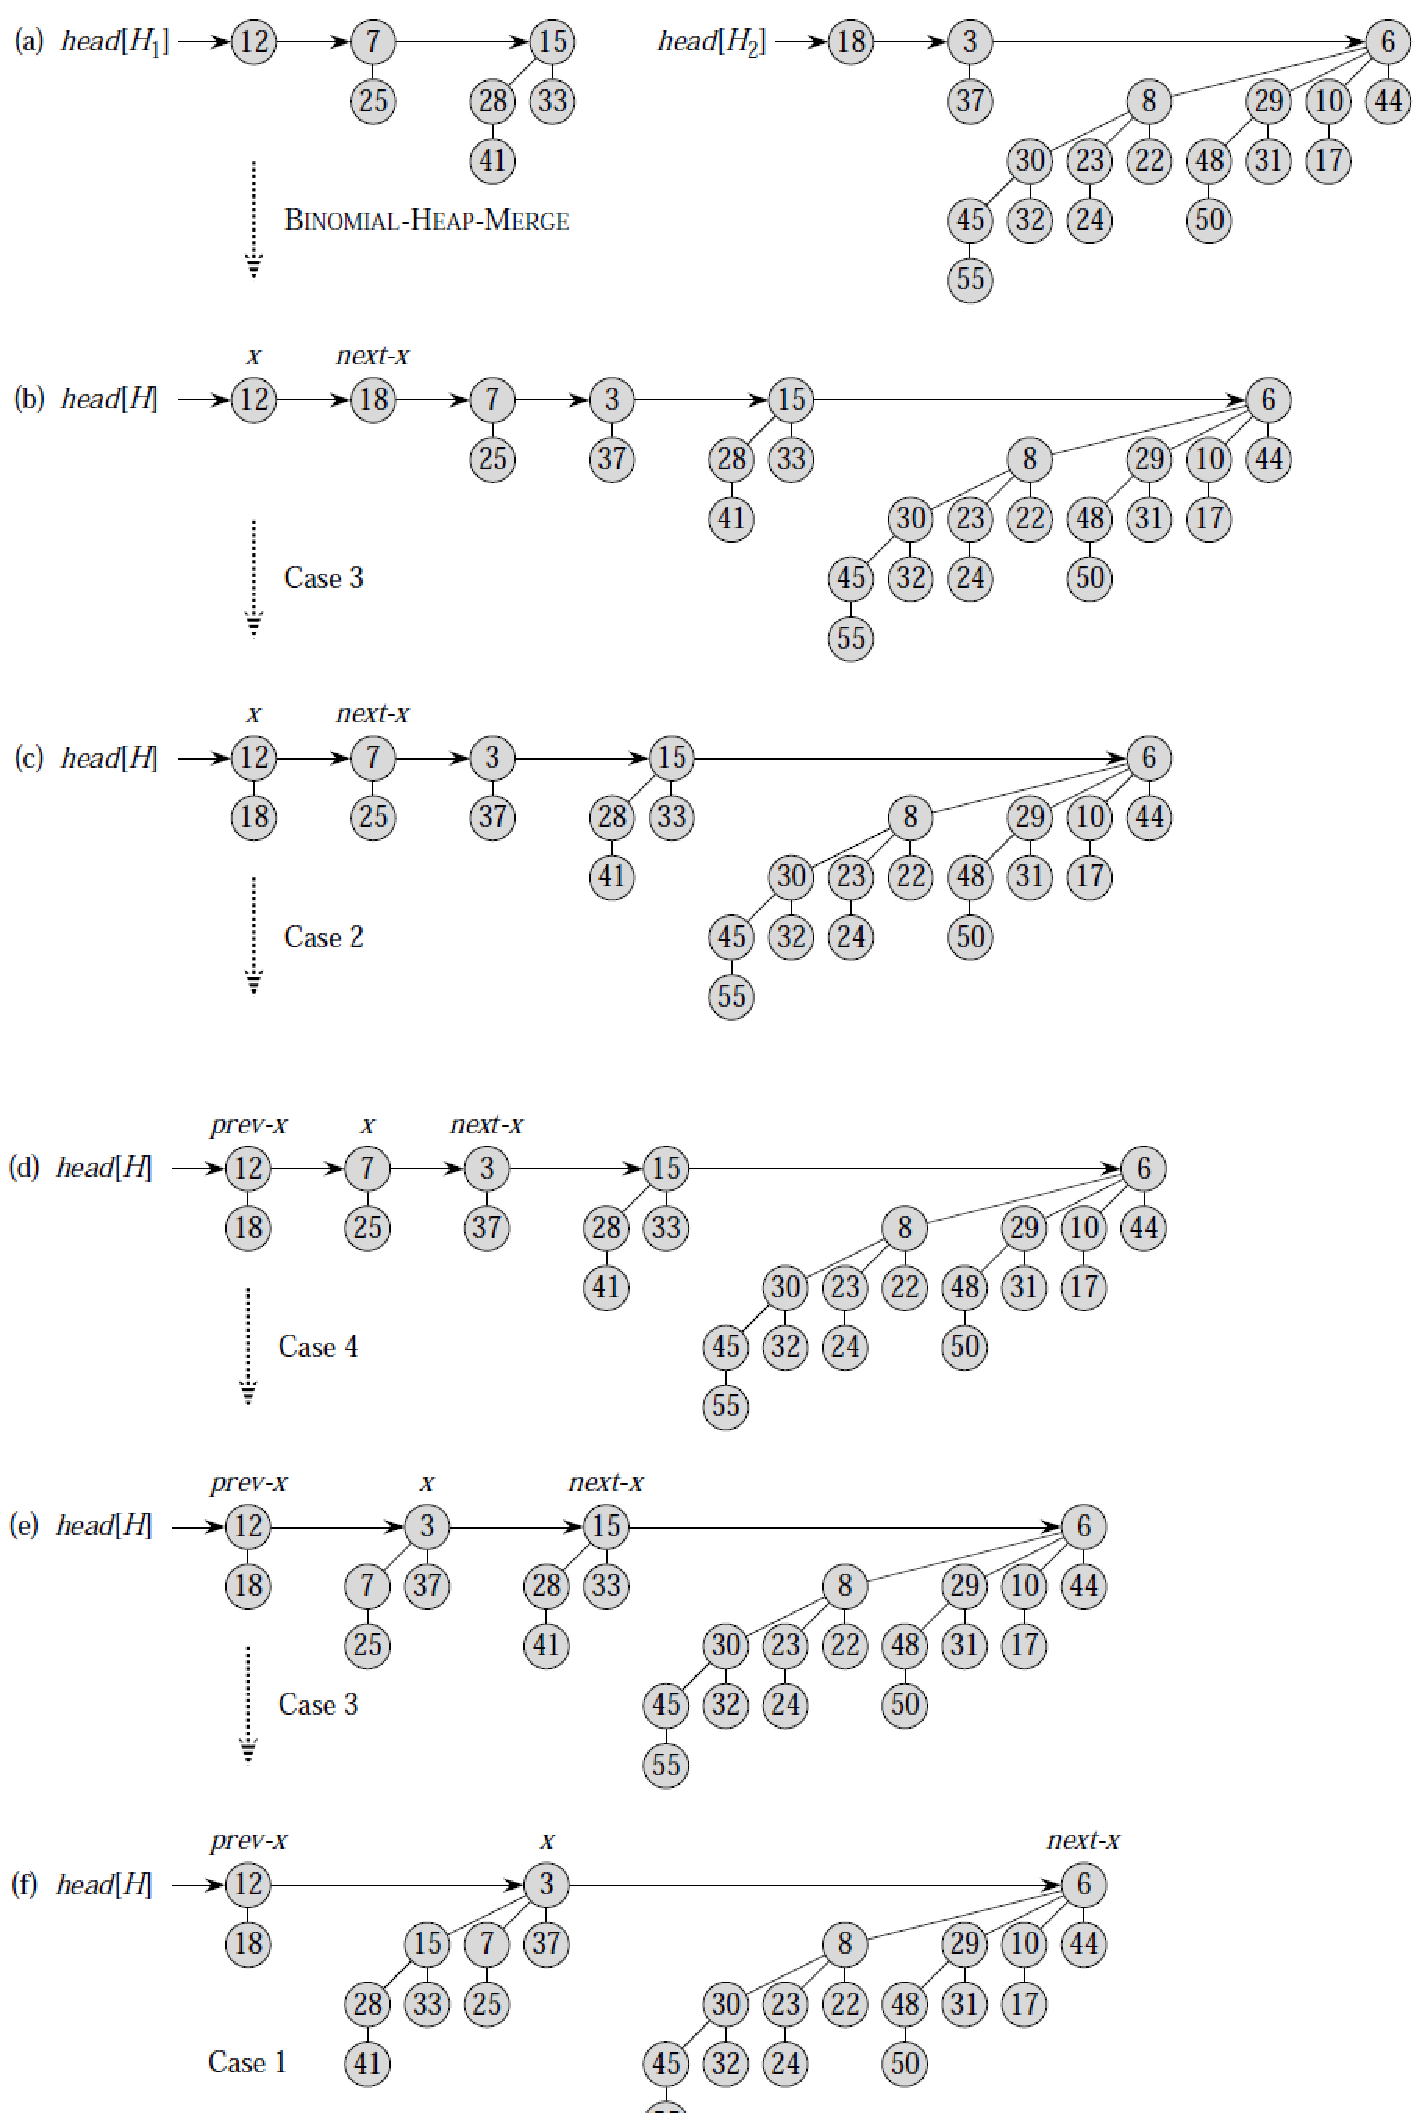
\includegraphics[scale = 0.23]{4.pdf}
 \end{figure}
\end{frame}




\end{document}
